%!TEX root = ../vortrag.tex
\section{Aufteilung auf Sequenzen}

\begin{frame}[t,fragile]{Aufteilung auf Sequenzen}
	\begin{itemize}
		\item sortiere Bilder nach Seriennummer der Kamera und Zeitpunkt der Aufnahme
		\item dafür notwendig: Zugriff auf die EXIF Maker Notes mit Hilfe des Programms \enquote{ExifTool} \cite{exif}
		\item unterteile die sortierte Folge von Bildern in Sequenzen, falls sich die Seriennummer ändert oder der Zeitunterschied zwischen zwei Bildern zu groß wird
		\item Umsetzung in Programm \enquote{Camera Trap Sequencer}:
			\begin{itemize}
				\item setzt viele nützliche Funktionen zum Aufteilen auf Sequenzen um
				\item GUI implementiert mit Qt 5
			\end{itemize}
	\end{itemize}
\end{frame}

\begin{frame}[t, fragile]{Camera Trap Sequencer}
	\begin{figure}
	\centering
	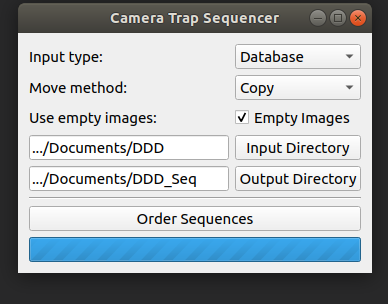
\includegraphics[scale=0.5]{img/CameraTrapSequencer.png}
	\caption{Grafische Benutzeroberfläche zur Aufteilung von Kamerafallensequenzen.}
	\end{figure}
\end{frame}